% #############################################################################
% This is Chapter 5
% !TEX root = ../main.tex
% #############################################################################
% Change the Name of the Chapter i the following line
\fancychapter{Implementation and Protocol}
\cleardoublepage
% The following line allows to ref this chapter
\label{chap:implementation}

This section builds on the system architecture. It will start by describing the communication protocols for each operation introduced in chapter \ref{chap:arch}, used in the implementation. The last section lists the standards and libraries chosen for the implementation. It finishes by outlining the implementation details, choices and their rationale.

% -----------------------------------------------------
% -----------------------------------------------------
\section{Protocol}\label{chap:implementation:protocol}

All data and operations will flow through a serial connection between the client software in the individual's computer and the physical box. A communications protocol needs to defined, in other for this communication to occur.
This section will explain and define the communication protocols between both the client application and the hardware device in detail. For each operation, it will describe its goal, the different phases, what data is traded in each phase and why.

% -----------------------------------------------------
\subsection{Initial State}\label{chap:implementation:protocol:initial-state}

The device will come from fabric configured and prepared with the necessary keys depending on two scenarios. In the simpler scenario, the device comes with the symmetric keys already shared and stored in each entities' device. They can begin to communicate immediately, with no setup necessary.
In the other scenario, the entities will receive the device with a pair of asymmetric keys, a private and public, generated inside the device from fabric. Each device will have the user's public keys, whom he wishes to communicate. The entity can request whose public keys he wants, before the device is initialized in fabric. This allows the users to share symmetric keys between them, which they can user to begin trading data securely.

All communications start with the client sending the operation code and receiving an "OK" message, meaning the user has access to the operation. If the user is not authenticated he receives a "NOT AUTHORIZED" message.
The authentication operation can always be be accessed by the user, all other operations can only be accessed after the user is authenticated.
Sending the operation code acts as a acknowledge message to check if the device is connected and powered to the computer.

% -----------------------------------------------------
\subsection{Authentication Protocol}\label{chap:implementation:protocol:auth}

Before executing any operation the user must authenticate himself to the device.
Figure~\ref{fig:protocol:authentication} depicts the authentication protocol.

%% ------------
\begin{figure}[h!]
	\centering     %%% not \center
	\subfigure[Authentication]{\label{fig:protocol:authentication}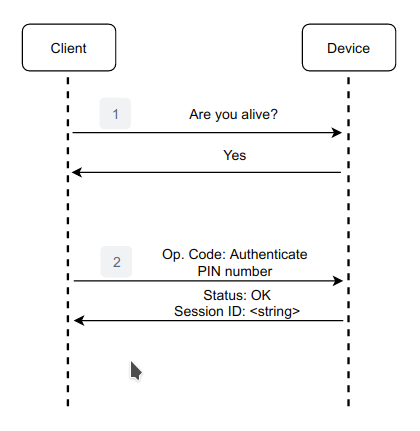
\includegraphics[width=70mm]{Images/authentication.png}}
	\subfigure[Change Authentication PIN]{\label{fig:protocol:change-PIN}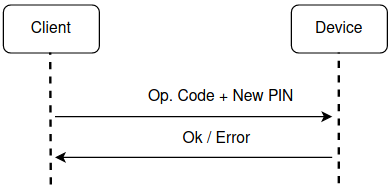
\includegraphics[width=70mm]{Images/change-PIN.png}}
	\caption{Authentication and PIN change protocols}
\end{figure}
% \begin{figure}[h!]
%         \centering
%         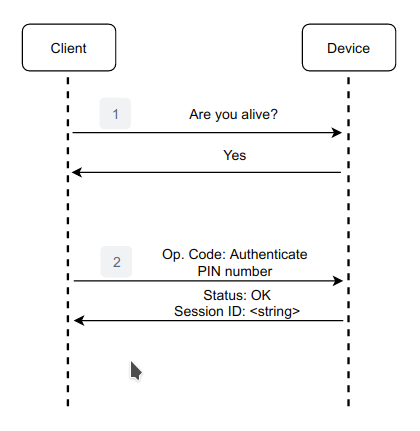
\includegraphics[width=0.4\textwidth]{./Images/authentication.png}
%         \caption{Authentication Protocol}
%         \label{fig:protocol:authentication}
% \end{figure}

The user initiates by sending a operation code. After the "OK" message, the user provides the device with the authentication \ac{PIN}. The device will respond with a authentication response parameter indicating failure or success. If successful, the session will be unlocked, allowing the user access to the main operations.

% -----------------------------------------------------
\subsection{Administration Protocol}\label{chap:implementation:protocol:admin}

There is only one administration operation, to change the authentication \ac{PIN}, pictured in figure~\ref{fig:protocol:change-PIN}.

% \begin{figure}[h!]
%         \centering
%         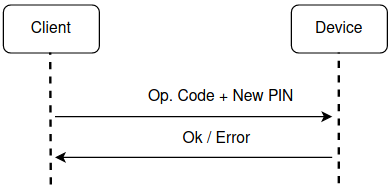
\includegraphics[width=0.4\textwidth]{./Images/change-PIN.png}
%         \caption{Protocol to Change Authentication PIN}
%         \label{fig:protocol:change-PIN}
% \end{figure}

After the operation code and received status message, the user sends the new \ac{PIN} number. The device responds with the status message of the operation.

% -----------------------------------------------------
\subsection{Secure Communications Protocol}\label{chap:implementation:protocol:comms}

The protocol for operations which secure communications will be defined here. It covers the encryption and authentication operation, which enables secure communications.% and non-repudiation through qualified digital signatures.
The protocol for secure data exchange illustrated in figure~\ref{fig:protocol:data-exchange} consists of four stages.

\begin{figure}[h!]
	\centering
	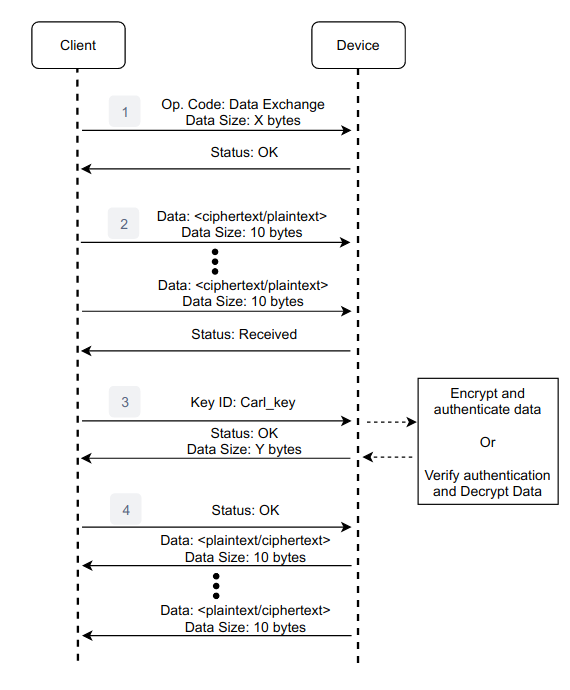
\includegraphics[width=0.55\textwidth]{./Images/data-exchange.png}
	\caption{Encryption+Authentication Protocol}
	\label{fig:protocol:data-exchange}
\end{figure}

The first stage is identical to all operations, the client sends the operation code and receives the authorization status. If he is not authorized, the user is required to authenticate first.
In the second stage the user client application sends the data size to be encrypted, waits for the "OK", and starts sending the data one block at a time.
A maximum of 16 bytes per message can be transmitted. Each message contains a part of the data and the size of the data in that packet. When the transmission ends, the device confirms its reception with an "OK" message.
In the third stage, the client software sends the ID of the symmetric key used to secure communications with.
In the final stage, after the box has finished the cryptographic operations, the device sends the result size to the client, waits for an "OK" message and sends the result. It consists of the encrypted data, MAC and IV.

The protocol to decrypt and authenticate is identical to the one pictured in figure~\ref{fig:protocol:data-exchange}. The device receives the ciphertext, \ac{MAC} and \ac{IV}, and returns the original plaintext data.

\hfill
\hfill

% The next protocols are relating to the generation and verification of digital signatures.
% The designed protocol for generation is represented in figure~\ref{fig:protocol:signature-generate}.
%% ------------
% \begin{figure}[h!]
%         \centering     %%% not \center
%         \subfigure[Generation Protocol]{\label{fig:protocol:signature-generate}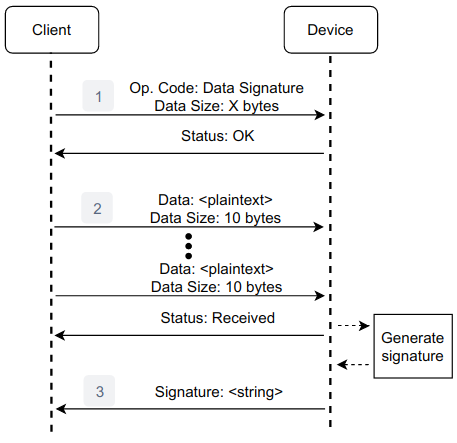
\includegraphics[width=79mm]{Images/signature-generate.png}}
%         \subfigure[Verification Protocol]{\label{fig:protocol:signature-verify}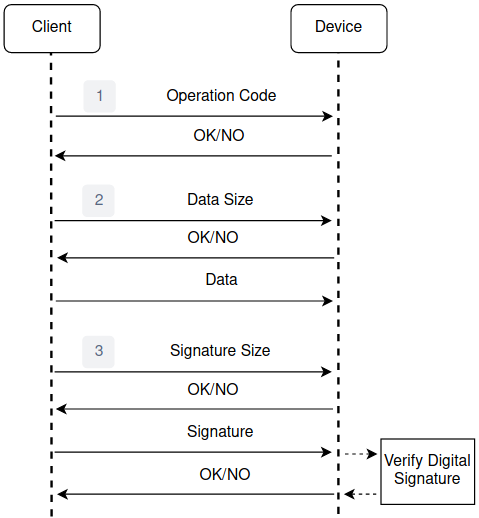
\includegraphics[width=79mm]{Images/signature-verify.png}}
%         \caption{Digital Signature Generation Protocols}
% \end{figure}

% The user initiates by sending the operation code and the plaintext data size.
% When the box responds with an OK message, the user transmits the data to be signed, one message at a time.
% In possession of the data, the device will generate the digital signature using the device's private key. When finished the signature is sent back to the user.
%
% The protocol for verifying digital signatures is pictured in figure~\ref{fig:protocol:signature-verify}.
% After the user sends the operation code, and the box responds with an OK message, the user transmits the data, used by the signer to generate the signature, one message at a time.
% When done, the user also sends the signature and the name of the signer, so the device knows what public key to use to verify the signature.
% Then, the device will verify the digital signature using the signer's public key, the data and the signature. The result will be sent back to the user.
%
% -----------------------------------------------------
\subsection{Communication Management Protocol}\label{chap:implementation:protocol:key}

The protocols for the communication management operations are detailed next, namely for symmetric key generation and key revocation. 
The protocol to generate a new symmetric key with another entity using asymmetric cryptography is detailed in figure~\ref{fig:protocol:ecdh}.

%% ------------
\begin{figure}[h!]
	\centering
	\subfigure[ECDH]{\label{fig:protocol:ecdh}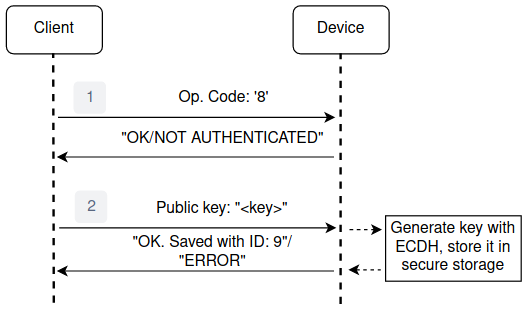
\includegraphics[width=79mm]{Images/ecdh.png}}
	\subfigure[Key Revocation]{\label{fig:protocol:delete-key}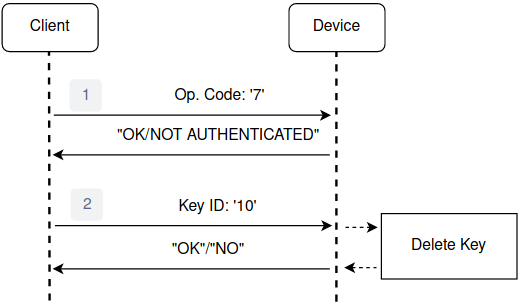
\includegraphics[width=79mm]{Images/delete-key.png}}
	\caption{Communication Management Protocols}
\end{figure}

After stage 1, the client forwards the entity's public key to the device, waits for an "OK" status, and sends the salt value. The device calls the ECDH algorithm with its private key and the received public key to generate a secret and run it through a key derivation function with the salt value to obtain the new symmetric key.
The new key is saved in secure storage with a new key id, which is returned to the client application.

The protocol for deleting an existing symmetric key from the device's secure storage is detailed in figure~\ref{fig:protocol:delete-key}.
After both sides trade operation code and OK status, the user sends the key ID, which identifies the symmetric key, and receives the operation status from the device after it has been deleted.

% -----------------------------------------------------
% -----------------------------------------------------
\section{Implementation}\label{chap:implementation:app}

This section contains all details about the developed implementation on the Hardware Security Module device.

% -----------------------------------------------------
\subsection{Libraries and Tools}\label{chap:implementation:app:tools}

The cryptographic software is running on the \ac{SoC} of a SmartFusion2 board from Microsemi, discussed in section~\ref{chap:background:computing:smartfusion}. It is an adequate device due to several components such as the required cryptographic functions in its system controller, a \ac{TRNG} essential for cryptography, secure storage for keys and anti-tampering protections.
The application was implemented using the C programming language, with the SoftConsole v3.4 \ac{IDE} and libraries of the board functionalities, provided by Microsemi. The configuration was generated using Libero v11.8. The device functions as a \ac{HSM}, connected through a \ac{USB} connection to a computer. It was programmed using the external FlashPro4 programmer required to develop and debug embedded applications with SoftConsole \cite{smartfusionSecurityPractices}.
The client software was also implemented in C, and is composed of a simple interface which allows communication through the cable, to the device.

% -----------------------------------------------------
\subsection{Cryptographic Algorithms}\label{chap:implementation:app:algorithms}

As previously mentioned, \ac{AES} is a popular symmetric-key standard. The security of \ac{AES}-\ac{GCM} in hardware is considered to be unsurpassed by any authenticated-encryption scheme~\cite{aesmodes}.
Unfortunately, the SmartFusion2 board, does not support this encryption algorithm. Therefore the solution implements a combination of an encryption algorithm with an authentication scheme. The board supports the \ac{AES} encryption modes for confidentiality, either 128 or 256 bits: \ac{ECB}, \ac{CBC}, \ac{OFB} and \ac{CTR}. CTR mode is the most favourable option because of its efficiency and security, assuming the IV is unique for each message.
For authentication, the board supports \ac{HMAC} with the \ac{SHA}-256 hash function, which uses a 256 bit symmetric key and generates a 256 bit code. For combining the CTR and HMAC algorithms, studies have shown that a combination of secure encryption and secure MAC must use the encrypt-then-MAC method~\cite{encryptmacorder}.
When choosing key sizes, taking into account the limited storage capacity of the board, a smaller, but still secure, key size is preferred. \ac{AES} guarantee both 128 and 256 bit security, with 128 and 256 bit keys. According to the \ac{NIST} recommendations~\cite{nistRecommendations}, algorithms which guarantee both 128 and 256 bit security, are expected to be secure from 2031 and beyond. \ac{AES}-128 is chosen, since it guarantees adequate security for the foreseeable future, and is the smaller option.

The system provides a single hash algorithm, \ac{SHA}-256, which has a security strength of 128 bits.
The \ac{HMAC}-\ac{SHA}-256 algorithm needs a 256 bit key, different from the one used with encryption, to ensure the best security practices. A 128 bit key can be used, if padded with zeros. Thus, for every communication, a 128 bit key for encryption and a 128 bit key for authentication is used. In total, a 256 bit shared secret.
The used algorithm for public-key cryptography is \ac{ECC} with 384 bit private and public keys, the only one supported by the board, which guarantees 192 bit security.

The qualified digital signatures operation combines \ac{ECC} and the \ac{SHA}-256 hash algorithm, and provides 128 bit security, calculated by taking the smallest security strength value of both algorithms. For the encryption and authentication operation combining \ac{AES}-128 and \ac{HMAC}-\ac{SHA}-256, 128 bit security is provided.

% -----------------------------------------------------
\subsection{Device Standardization}\label{chap:implementation:standards}

The solution should support a plethora of devices, as it will increase the adoptability of the solution among clients. This entails the use of a widely established protocol, which clearly defines a set of functions and standards the system should follow.
The \ac{PKCS} \#11 standard will be utilized to fulfill this requirements. It allows operations to be standardized across different devices, increasing the range of supported devices. By implementing the system in accordance with these guidelines, it will have a higher device interoperability. Additionally, it allows the application to use, create and modify objects, without exposing them to its memory.

